\documentclass[12pt]{article}

\setlength{\parindent}{0em}
\setlength{\parskip}{.5em}

\usepackage{framed}
\newcounter{problem}
\newcounter{problempart}[problem]
\newcounter{solutionpart}[problem]
\newenvironment{problem}{\stepcounter{problem}\noindent{\bf\arabic{problem}.}}{\setcounter{problempart}{0}\setcounter{solutionpart}{0}}
\newenvironment{solution}{\par\textcolor{green!50!black}\bgroup}{\egroup\par}
\newcommand{\qpart}{\stepcounter{problempart}${}$\\\noindent{(\alph{problempart})} }
\newcommand{\spart}{\stepcounter{solutionpart}${}$\\\noindent{(\alph{solutionpart})} }
\newcommand{\TODO}{\textcolor{red}{$\blacksquare$}}
\newcommand{\SOL}[1]{\textcolor{green!50!black}{#1}}

\usepackage{hyperref}
\usepackage{fullpage}
\usepackage{amsmath,mathabx,MnSymbol}
\usepackage{color,tikz}
\usepackage{pstricks}
\usepackage{pst-plot,pst-node}
\usepackage{footnote,enumitem}
\usepackage{longtable}
\newcommand{\mx}[1]{\begin{pmatrix}#1\end{pmatrix}}
\definecolor{dkgreen}{rgb}{0,.5,0}
\usepackage{algorithm}
\usepackage[noend]{algpseudocode}

\newcommand{\uu}{\mathbf{u}}
\newcommand{\vv}{\mathbf{v}}
\newcommand{\cc}{\mathbf{c}}
\newcommand{\ww}{\mathbf{w}}
\newcommand{\xx}{\mathbf{x}}
\newcommand{\zz}{\mathbf{z}}
\newcommand{\ee}{\mathbf{e}}
\newcommand{\pp}{\mathbf{p}}
\newcommand{\qq}{\mathbf{q}}
\renewcommand{\AA}{\mathbf{A}}
\newcommand{\BB}{\mathbf{B}}
\newcommand{\nn}{\mathbf{n}}
\newcommand{\gp}[1]{\left(#1\right)}

\newcommand{\TODOL}[1]{\textcolor{red}{\underline{\hspace{#1 cm}}}}

\usepackage{listings}

\lstset{
  language=C++,
  showstringspaces=false,
  identifierstyle=\color{magenta},
  basicstyle=\color{magenta},
  keywordstyle=\color{blue},
  identifierstyle=\color{black},
  commentstyle=\color{green},
  stringstyle=\color{red}
}

\begin{document}

\title{CS130 - LAB - Bresenham's line algorithm / midpoint algorithm}
\date{}
\author{Name: \TODOL7\qquad\qquad SID: \TODOL4}
\maketitle
\begin{center}
\end{center}

\section{Midpoint algorithm - case 1: $0 \le m \le 1$}

This Lab consists of implementing the midpoint algorithm to draw continuous
lines using only integer operations. Recall the line equation is $y = mx + n$,
where $m$ is the slope and $n$ is the $y$ intercept.  Given two points $p_0 =
(x_0, y_0)$ and $p_1 = (x_1, y_1)$, the slope is calculated as $m = \frac{y_1 -
  y_0}{x_1 - x_0} = \frac{dy}{dx}$.  Consider $0 \le m \le 1$ (line in angle
between 0 and 45 degrees).  The idea is to determine which of the two pixels
($a$ or $b$) we should draw. Complete the missing coordinates of the points
below.\\
\begin{center}
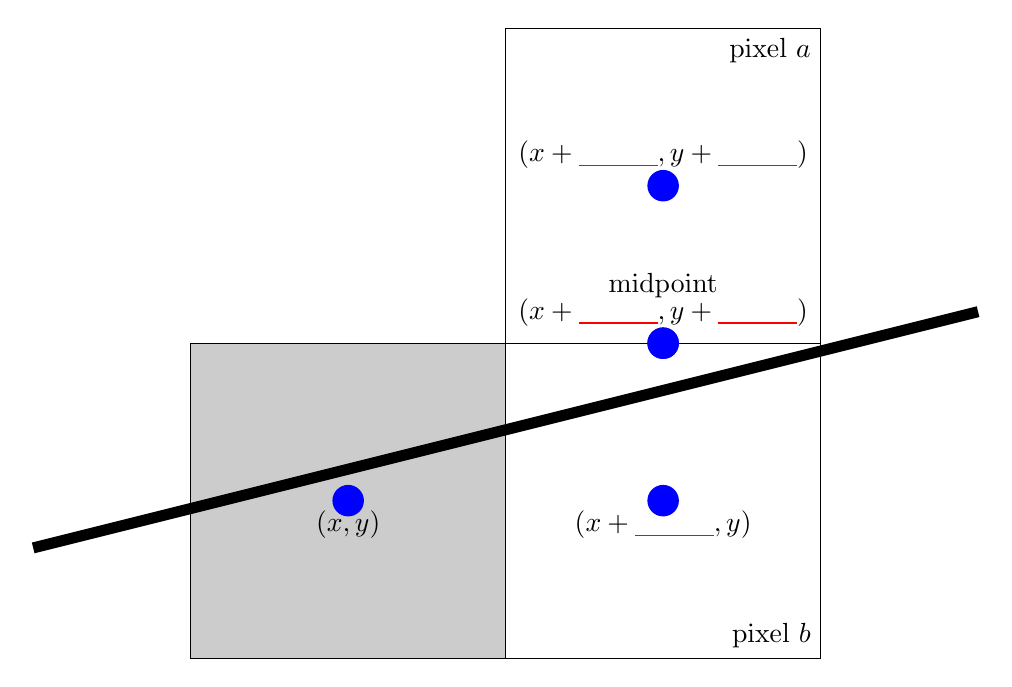
\begin{tikzpicture}[scale=2]
\draw[fill=black!20] (0,0) rectangle (2,2);
\draw[] (2,0) rectangle (4,2);
\draw[] (2,2) rectangle (4,4);
\draw[fill=blue,draw=none] (1,1) node[below]{$(x,y)$} circle (.1);
\draw[fill=blue,draw=none] (3,1) node[below]{$(x+\TODOL1  ,y)$} circle (.1);
\draw[fill=blue,draw=none] (3,3) node[above,inner sep=6]{$(x+\TODOL1,y+\TODOL1)$} circle (.1);
\draw[fill=blue,draw=none] (3,2) node[above,inner sep=6]{$(x+\TODOL1,y+\TODOL1)$} circle (.1);
\draw[fill=blue,draw=none] (3,2) node[above,inner sep=6+1em]{midpoint} circle (.1);
\node[above left] at (4,0) {pixel $b$};
\node[below left] at (4,4) {pixel $a$};
\draw[line width=4] (-1,.7) -- (5,2.2);
\end{tikzpicture}
\end{center}

In particular, we can evaluate the midpoint between $a$ and $b$ using a function
$f(x,y)$ that returns a positive number if the point $(x,y)$ lies above the
line, negative if it lies below, and zero if the point is on the line.  This
function should have the form
\begin{align}\label{eqn:fxy}
f(x, y) = A x + B y + C,
\end{align}
where $A$, $B$, and $C$ depend on $x_0$, $y_0$, $x_1$, and $y_1$.  You may
assume that $x_0 \le x_1$, $y_0 \le y_1$, and that the slope satisfies $0 \le m
\le 1$.  (If the endpoints are in the opposite order, you can swap them before
you rasterize.)  Note that scaling $A,B,C$ by a positive number does not change
the sign of $f(x,y)$, so we can require that $A,B,C$ be polynomials.  (Hint: use
$f(x_0,y_0) = f(x_1,y_1) = 0$ to solve for $B$ and $C$ in terms of $A$ and the
endpoints.  Choose $A$ so that the fractions go away and so that $A,B,C$ share
no common factors.  At this point, your $f(x,y)$ should be correct up to sign.
Since points above the line should give you a positive value, you can check
$f(x_0,y_0+1) > 0$, since the point $(x_0,y_0+1)$ should be above the line.  If
the sign is wrong, negate $A,B,C$.)
$A = \TODOL7, B = \TODOL7, C = \TODOL7$.

In the diagram above, we have just finished setting the pixel $(x,y)$, and now
we must decide whether we should increment $y$, leading us to either pixel $a$
or $b$.  Let $g(x,y)$ be a function that is negative if we want to increment
$y$.  You can use $f(x,y)$ to help you define $g(x,y)$.  (Note that $f(x,y) \ne
g(x,y)$.  If $x,y$ are integers, $g(x,y)$ should an integer, too.  Note that you
can scale it to clear fractions, since only the sign matters.)  $g(x,y) =\TODOL9$.



This would be a good time to implement a version of \texttt{draw\_line} to make
sure that all of the work that you have done so far is correct.  Your code
should work correctly when $0 \le m \le 1$.  (In other cases, it may do strange
things - we will handle the other cases later.)  When it works, continue on to
the next step. At this stage, your code should look like this:
\begin{lstlisting}
void draw_line(int x0, int y0, int x1, int y1, float col[3])
{
    /* TODO: swap the points? */
    for(int x=x0,y=y0;x<=x1;x++)
    {
        set_pixel(x,y,col);
        int g=/* TODO */;
        if(g<0) y++;
    }
}
\end{lstlisting}

\section{Case 2: $-1 \le m \le 0$.}

Next, we will extend our algorithm to handle slopes $-1 \le m \le 0$.  Instead
of updating $x,y$ using \texttt{x++;} and \texttt{y++;}, we will instead use
\texttt{x++;} and \texttt{y+=dy;}, where $\Delta y = \pm 1$.  The points
$(x_0,y_0)$ and $(x_1,y_1)$ should be swapped if \TODOL6.Next, we need to compute $\Delta y = \TODOL6$ (from $x_0, x_1, y_0, y_1$).

Now, we must update our definition of $g(x,y)$ so that it works correctly when
$\Delta y = 1$ or $\Delta y = -1$.  We must make sure that $g(x,y)<0$
when we want to change $y$ and $g(x,y) \ge 0$ when we want to leave $y$
unchanged.  $g(x,y) = \TODOL9$.

This is a good time to test your modifications.  At this stage, your code should
look like this:
\begin{lstlisting}
void draw_line(int x0, int y0, int x1, int y1, float col[3])
{
    /* TODO: swap the points? */
    int dy=/* TODO: this should be +1 or -1. */;
    for(int x=x0,y=y0;x<=x1;x++)
    {
        set_pixel(x,y,col);
        int g=/* TODO */;
        if(g<0) y+=dy;
    }
}
\end{lstlisting}

\section{Incremental updates.}

Instead of recomputing $g$ each iteration, we instead like to update it
incrementally.  If $g<0$, then we will update \texttt{x++;y+=dy;g+=dg0;}.
Otherwise, we will update \texttt{x++;g+=dg1;}.  The initial value of $g$ should
be $g = \TODOL6$.  The update increments are $\Delta g_0 = \TODOL6$ and $\Delta
g_1 = \TODOL6$.  (You can compute the increments by writing down the difference
between what $g$ is currently and what it should be in the next iteration
assuming the corresponding update has been applied.  This difference should be
the same for every loop iteration.)

This is a good time to test your modifications.  At this stage, your code should
look like this:
\begin{lstlisting}
void draw_line(int x0, int y0, int x1, int y1, float col[3])
{
    /* TODO */
    int dy=/* TODO: this should be +1 or -1. */;
    int g=/* TODO */;
    int dg0=/* TODO */;
    int dg1=/* TODO */;
    for(int x=x0,y=y0;x<=x1;x++)
    {
        set_pixel(x,y,col);
        if(g<0)
        {
            y+=dy;
            g+=dg0;
        }
        else g+=dg1;
    }
}
\end{lstlisting}

\section{Cases 3 \& 4: $|m|>1$}

The remaining cases can be handled by swapping the roles of $x$ and $y$ in your
existing code.  (You do not need to repeat all of your derivations.  This step
should be very easy.)

Your final code should look like this:
\begin{lstlisting}
void draw_line(int x0, int y0, int x1, int y1, float col[3])
{
    if(/* TODO */)
    {
        /* TODO */
        int dy=/* TODO: this should be +1 or -1. */;
        int g=/* TODO */;
        int dg0=/* TODO */;
        int dg1=/* TODO */;
        for(int x=x0,y=y0;x<=x1;x++)
        {
            set_pixel(x,y,col);
            if(g<0)
            {
                y+=dy;
                g+=dg0;
            }
            else g+=dg1;
        }
    }
    else
    {
        /* TODO */
        int dx=/* TODO: this should be +1 or -1. */;
        int g=/* TODO */;
        int dg0=/* TODO */;
        int dg1=/* TODO */;
        for(int y=y0,x=x0;y<=y1;y++)
        {
            set_pixel(x,y,col);
            if(g<0)
            {
                x+=dx;
                g+=dg0;
            }
            else g+=dg1;
        }
    }
}
\end{lstlisting}

\end{document}
